\documentclass{article}
\usepackage{graphicx,caption}


\graphicspath{ {graphs/} }

\usepackage{geometry}
\geometry{legalpaper,  margin=1.0in}

\usepackage{Sweave}
\begin{document}
\Sconcordance{concordance:shrub_writeup.tex:shrub_writeup.Rnw:%
1 9 1 1 0 19 1}

Within individual woody plants are flower and leaf phenophases initiated by the same cues? If so, we would expect to see the lag between leaf and flower pheonophases remain relatively constant even as cues change. 

\begin{figure}[h!]

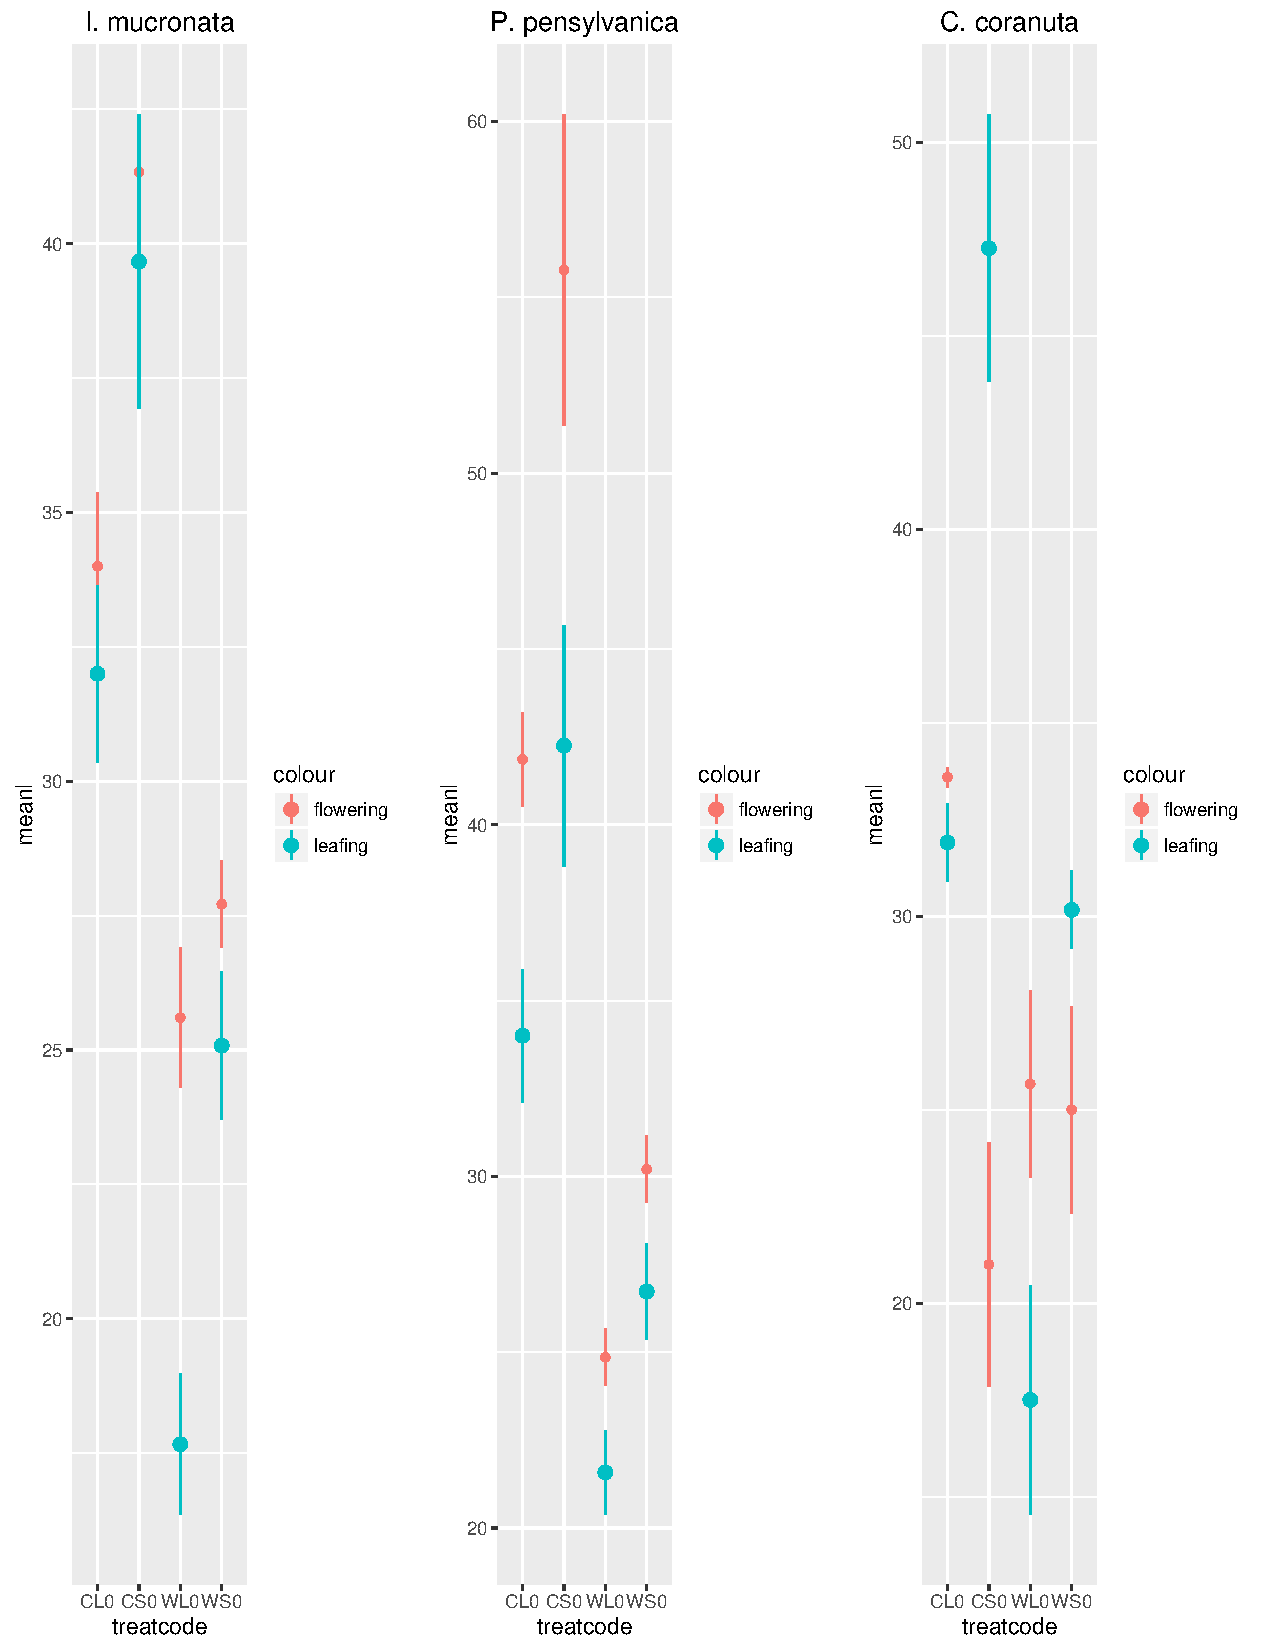
\includegraphics[width=15cm, height=12cm]{shrubs_sidebyside.pdf}\\
\caption{Mean first flower and mean leafout plotted by cue treatments for three deciduous shrubs}
\end{figure}
Of particular interest, the we see that under when exposed to short photoperiod, \textit{Corylus coranuta} switches between seranthy and proteranthy
\begin{figure}[h!]
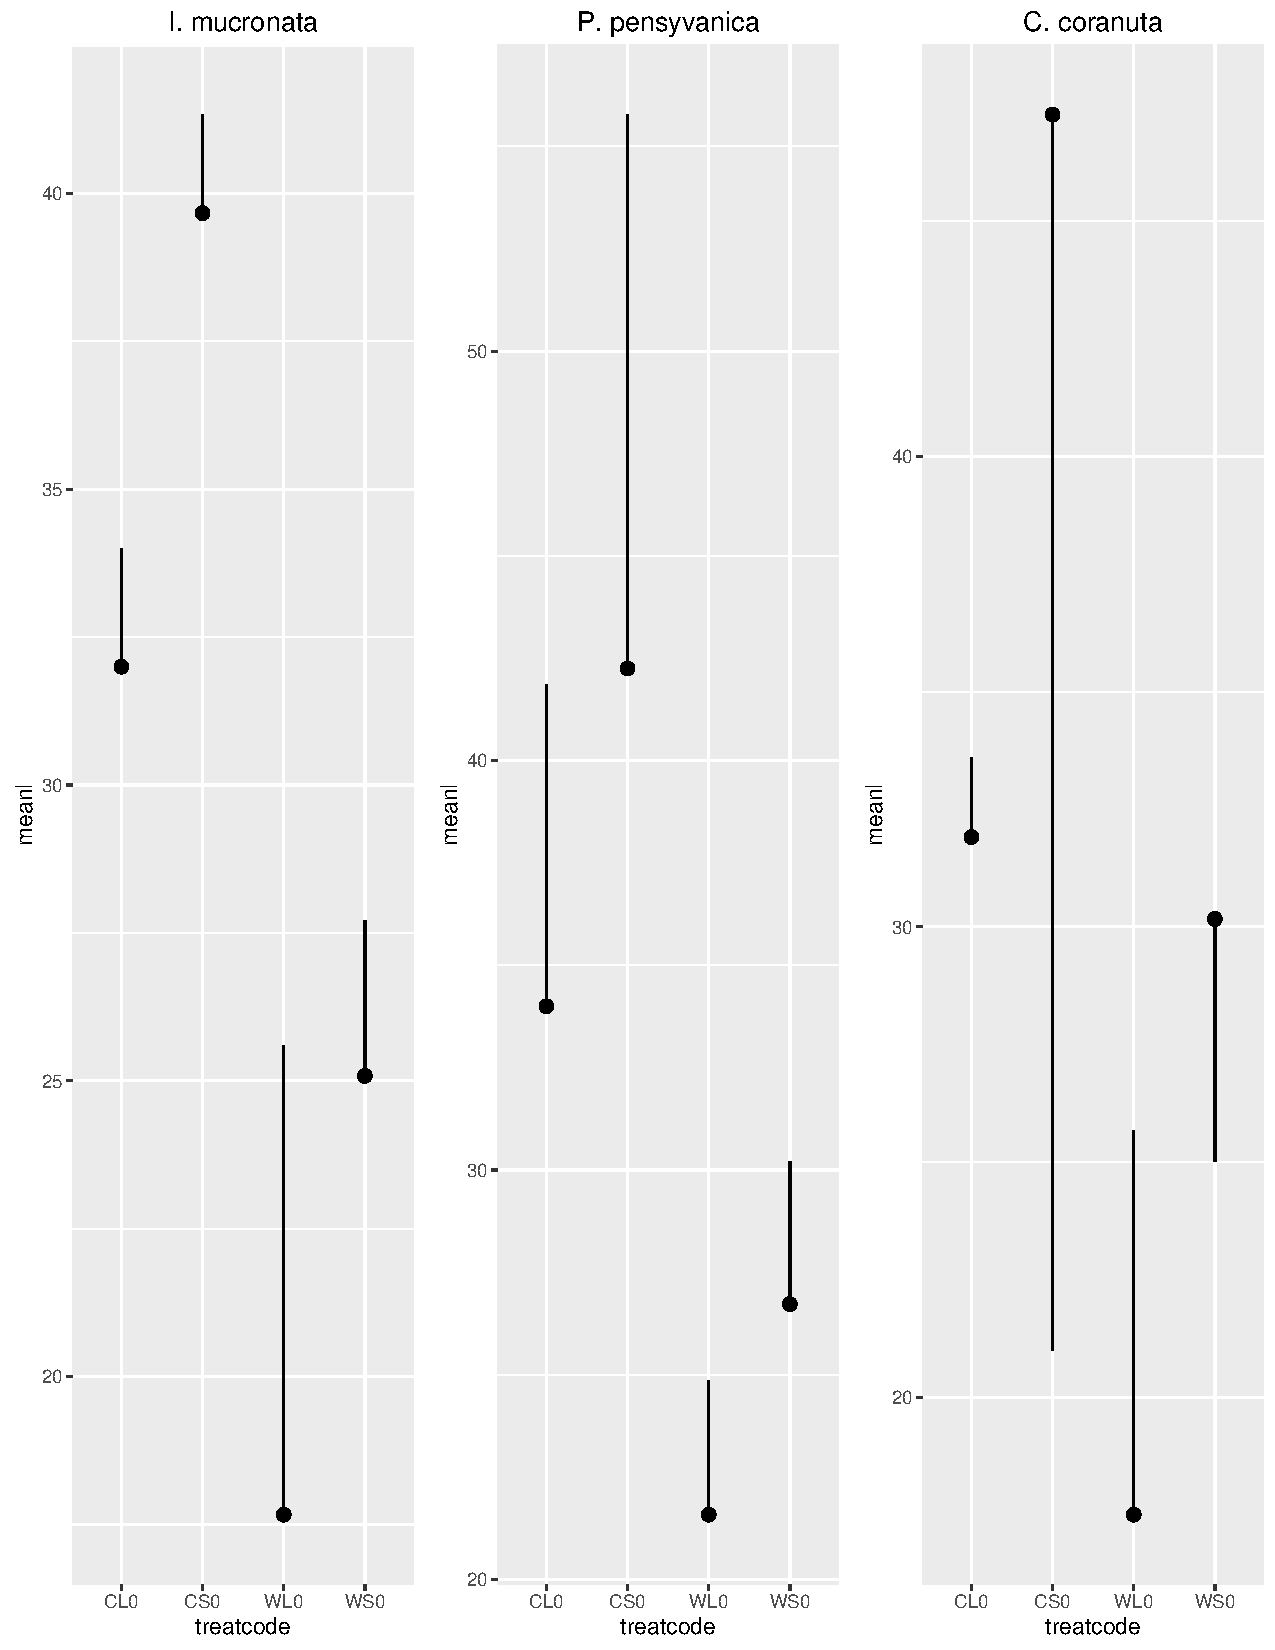
\includegraphics[width=14cm, height=12cm]{shrub_spread_graphs.pdf}
\caption[width=10cm]{The temporal offset between mean first flower and mean leafout by cue treatment for 3 deciduous species. The solid points 
$\bullet$
show mean leafout and the open ends of lines
$\mid$ 
mean first flower}
\end{figure}

\end{document}
